\section{Experiments Results and Analysis}

\subsection{Hypothesis 1}

This comparison is done between Khoi's SARSA algorithm, and Airi's Q-Learning algorithm. Below is the graph of average reward
for each algorithm, with $\epsilon$ kept static at 0.5

\begin{figure}[H] %h forces the figure to be inserted right here
    \centering
    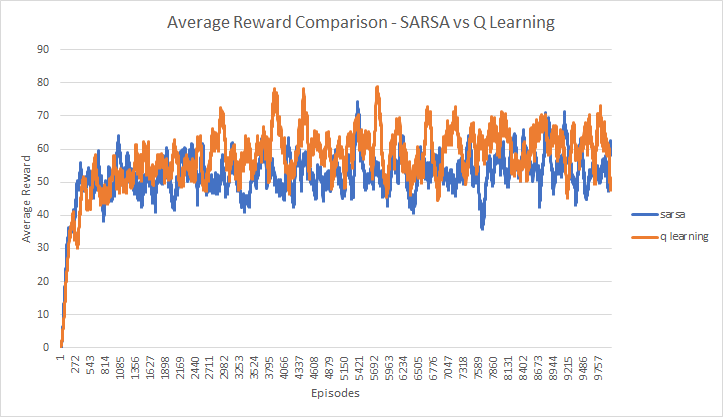
\includegraphics[width=0.7\linewidth]{sarsa-vs-ql.png}
    \caption{Comparison of SARSA and Q Learning}
\end{figure}

Looking at the figures, we can see that Q-Learning perform slightly better than SARSA, as the average reward stayed at a higher range for longer.
Moreover, Q-Learning has an average reward of $57.44$ while SARSA's average is only $52.41$.

\subsection{Hypothesis 2}

We explored three different methods of $\epsilon$ decay. First, $\epsilon$ is kept static at a value of 0.5. Second, 
$\epsilon$ followed the decaying function of $\epsilon = 0.5 * \frac{1}{no. of episodes}$. Finally,
$\epsilon$ follows the exponential decaying function of $\epsilon = 0.5 * e^{-0.001*no. of episodes}$

For SARSA, comparing the three methods of $\epsilon$ decay, yields the following results:

\begin{figure}[H] %h forces the figure to be inserted right here
    \centering
    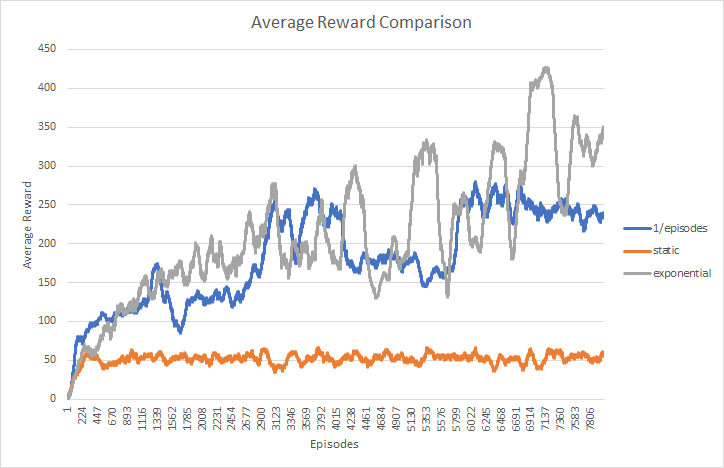
\includegraphics[width=0.75\linewidth]{epsilon-decay-comparison.png}
    \caption{Average Reward of SARSA, Comparing Different $\epsilon$ Decay}
\end{figure}

Additionally, the mean and standard deviation for each method are as follows:

\begin{table}[H]
    \begin{tabular}{lll}
    \hline
    Method      & Mean   & Standard Deviation \\ \hline
    Static      & 52.41  & 7.089              \\
    1/Episodes  & 116.56  & 45.775             \\
    Exponential & 192.32 & 68.383             \\ \hline
    \end{tabular}
    \caption{Mean of Average Reward and Standard Deviation}
\end{table}

As these results show, for the SARSA algorithm, exponential decay of $\epsilon$ performed the best.

\subsection{Hypothesis 3}

For Q Learning, in addition to the three different methods of $\epsilon$ decay mentioned above, Airi implemented a softmax policy. It chooses an action $\alpha$ from all actions \textit{A} based on the probability determined by a softmax function, which is $   \frac {e^{\frac{Q(a)}{\tau}}}{\sum_{b \in A}\cdot e^{\frac{Q(b)}{\tau}}} \cdot $ where $\tau$ is temperature parameter used to control the randomness of predictions and Airi sets $\tau$  = 0.1 for this experiment. 

Here are the comparison graph and table:

\begin{figure}[H] %h forces the figure to be inserted right here
    \centering
    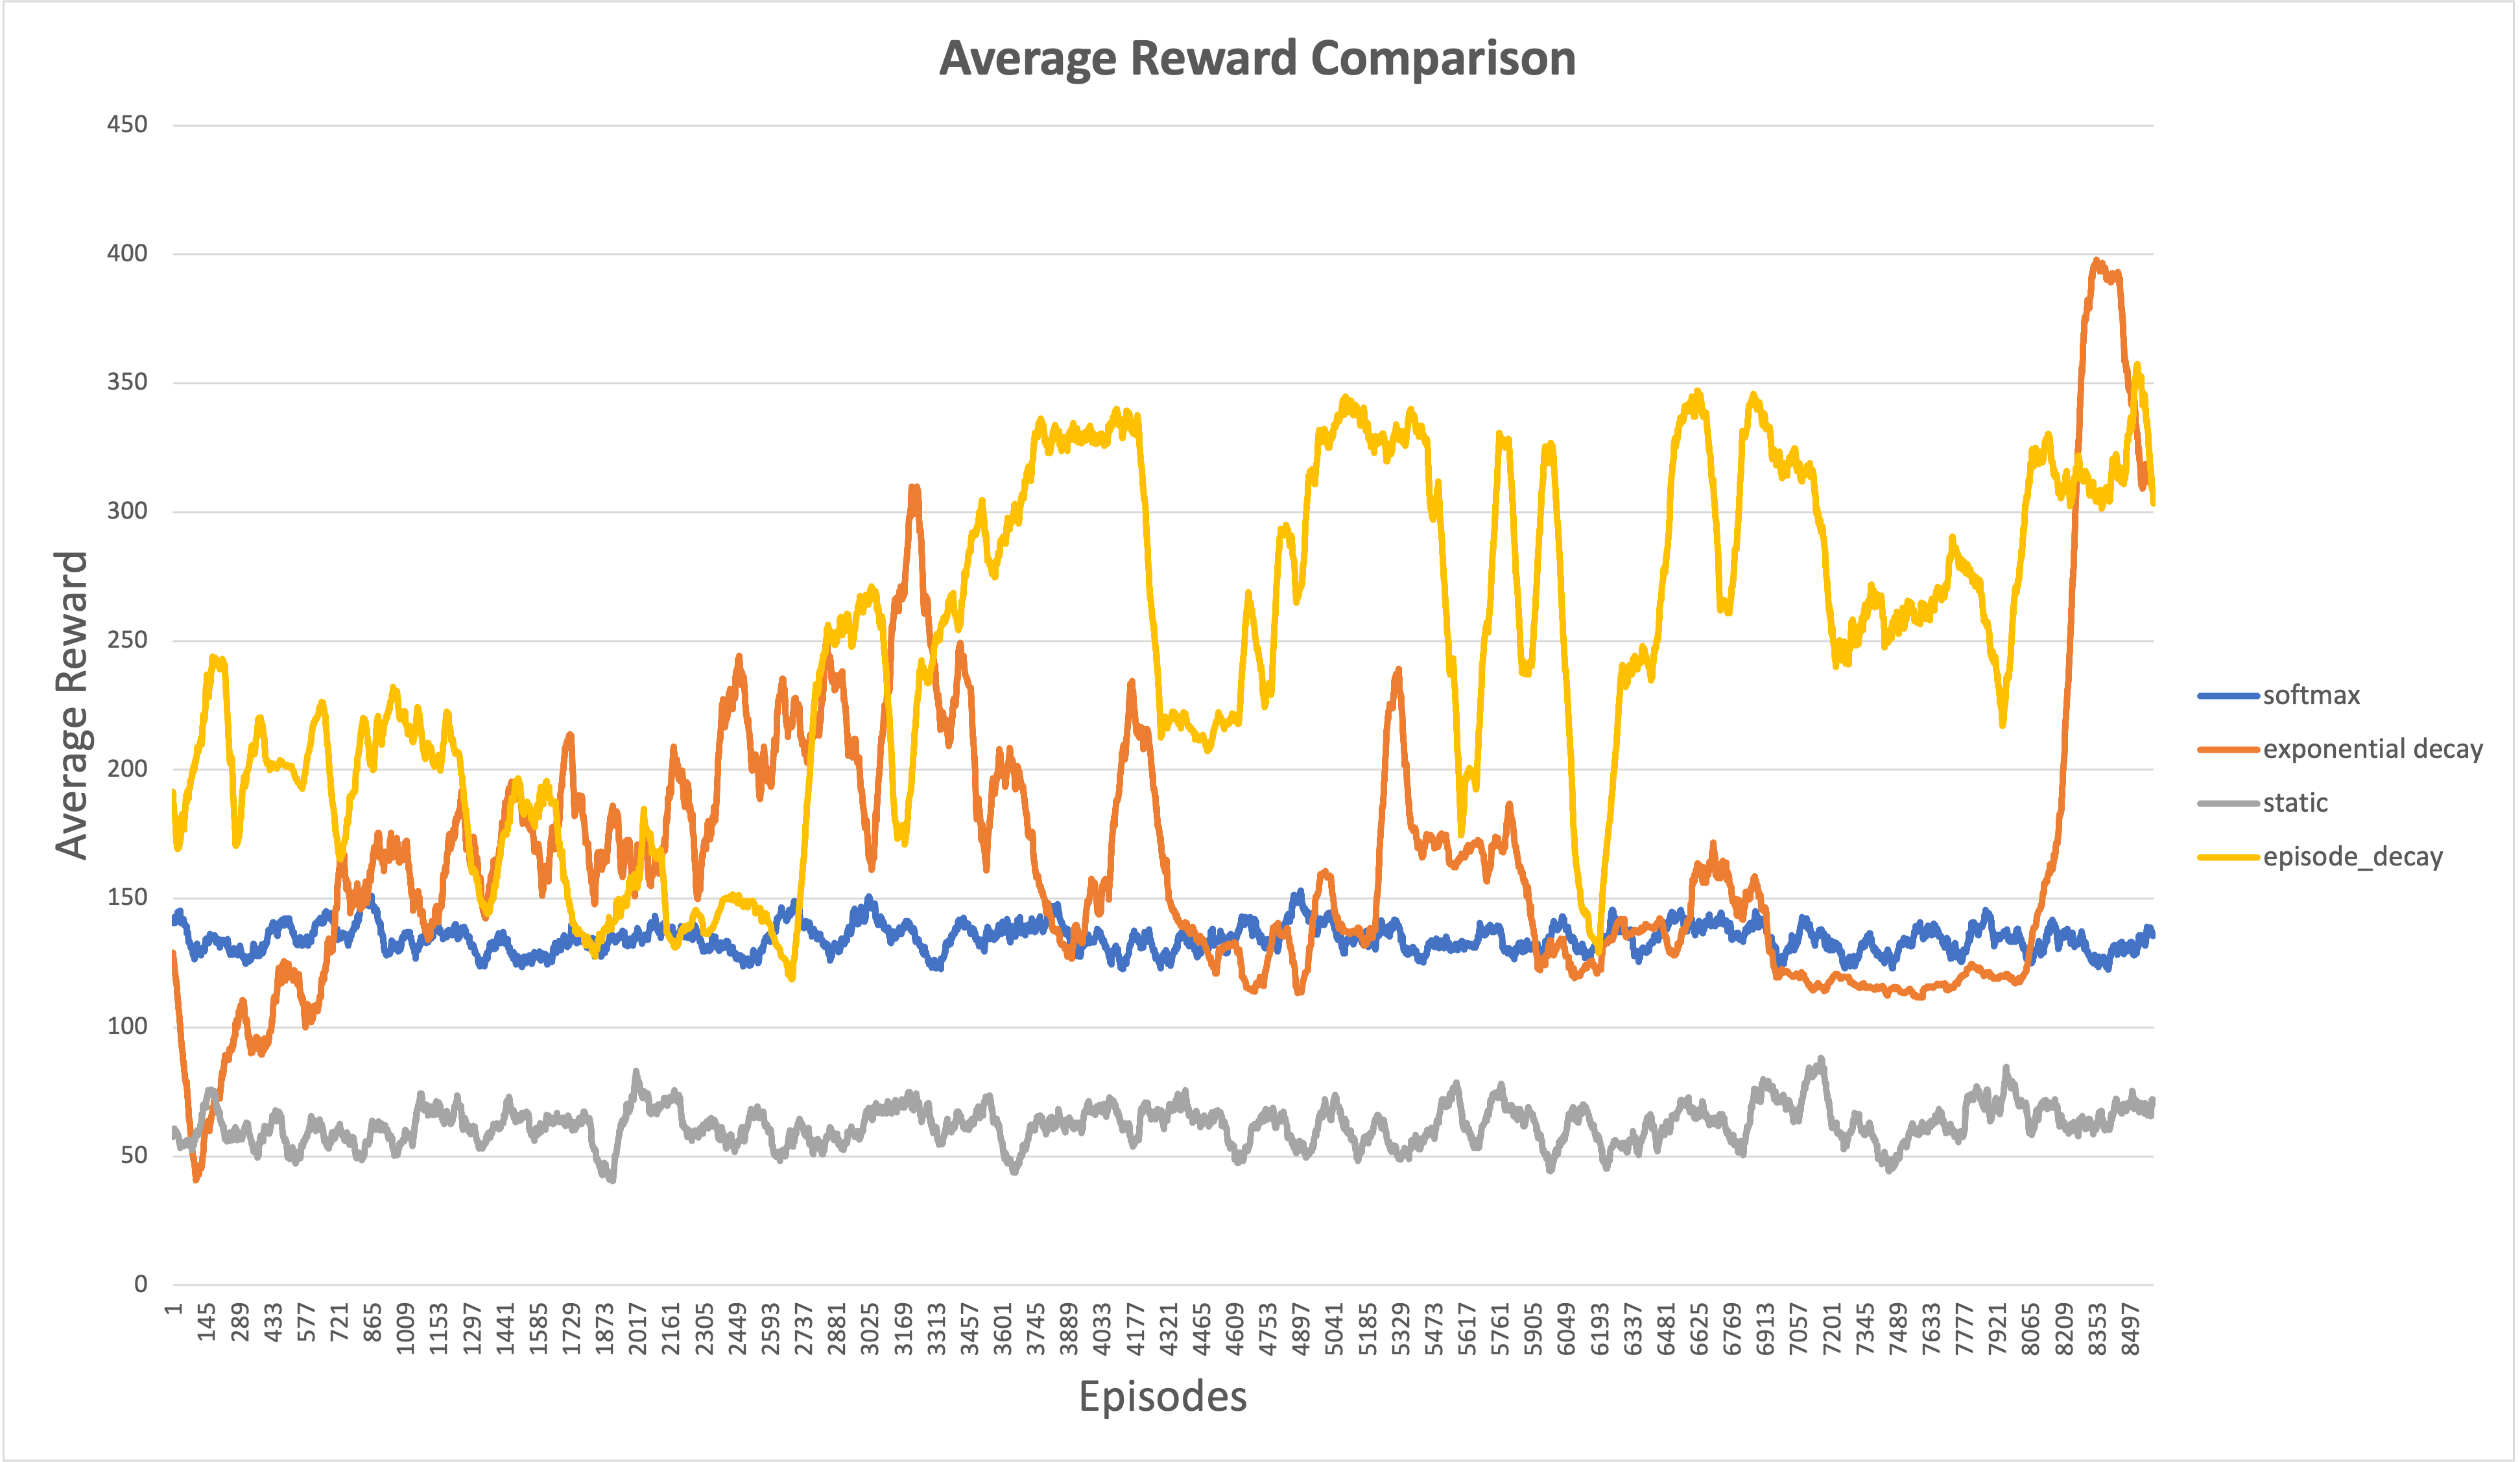
\includegraphics[width=0.75\linewidth]{comp_result.png}
    \caption{Average Reward of Q-Learning, Comparing $\epsilon$ Greedy and Softmax}
\end{figure}

\begin{table}[H]
\centering
\begin{tabular}[t]{lcc}
\toprule
& Mean &Standard Deviation\\
\midrule
Static & 61.35 &7.6\\
1/Episodes & 194.52 & 68.62\\
Exponential & 177.71 & 52.26\\
Softmax & 133.88 & 6.94\\
\bottomrule
\end{tabular}
\caption{Mean of the Average Reward and Standard Deviation.}
\end{table}%

From the above table and graph, we can see that the mean of average reward for episode decay is higher than exponential decay, but exponential decay managed to reach a higher maximum mean of average reward. Furthermore, softmax did not perform well when compared to the two $\epsilon$ decay methods, but it performed better than keeping $\epsilon$ static at 0.5.